\immediate\write18{makeindex -s nomencl.ist -o "\jobname.nls" "\jobname.nlo"}

% Relatório técnico da disciplina Tópicos Avançados em Inteligência
% Artificial I -- Especialização em Inteligência Artificial Aplicada (IFG)
\documentclass[relatorio]{formatacao/classe-ifg}
% Opções da classe-ifg (ao usar mais de uma, separe por vírgulas):
%   [tese]  	              	-> Tese de doutorado.
%   [dissertacao]     	-> Dissertação de mestrado (padrão).
%   [monografia]     	-> Monografia de especialização.
%   [tcc]   	              	-> Trabalho de conclusão de curso (graduação).
%   [qualificacaom]  	-> Qualificação de mestrado.
%   [qualificacaoe]   	-> Qualificação de especialização.
%   [qualificacaot]   	-> Qualificação de TCC.
%   [preprojetom]   	-> Pré-projeto de mestrado.
%   [preprojetoe]    	-> Pré-projeto de especialização.
%   [preprojetot]    	-> Pré-projeto de TCC.
%   [relatorio]    		-> Relatório de disciplina.

% Caso precise, corrija hifenização aqui
\hyphenation{mo-no-gra-fi-a pro-ces-so}

%INICIO DO DOCUMENTO ---------------------------------------------- %
\begin{document}




% EDITAR - Todos os cursos  ------------------------------------------- %
% -------- Autor(es)
\autor{Igor Coutinho Ferreira Nobre}
% -------- Título e subtitulo
\titulo{Data Warehouse Organizacional e Data Marts}
\subtitulo{Integração das bases Northwind e Mercearia, modelagem dimensional}
% -------- Curso
\tipocurso{Especialização}
\curso{Inteligência Artificial Aplicada}
% Inserir apenas no caso de relatório de disciplina
\disciplina{Tópicos Avançados em Inteligência Artificial I}
% -------- Local e data
\campus{Goiânia} % Câmpus em foi desenvolvido o trabalho
\dia{29} % Data de entrega do relatório
\mes{09} % Formato numérico: \dia{01}, \mes{01} e \ano{2007}
\ano{2026} %
% -------- Orientador(a)
\orientador{Dr. Sirlon Diniz de Carvalho}



% NÃO EDITAR. Se necessário edite apenas os arquivos na pasta "pre" %
\capa
\termo
\rosto % Primeira folha interna do trabalho
\ficha
\aprovacao
% Para o tipo [relatorio], \tabelas chama \cresumopre internamente ao
% final (independente do que foi passado nas opções), compondo o Resumo a
% partir de pre/preResumo.tex. Este relatório não usa Resumo; a linha
% abaixo neutraliza essa chamada sem alterar a classe-ifg.
\renewcommand{\cresumopre}{}
\tabelas
\cleardoublepage
\tableofcontents
\cleardoublepage



% EDITAR - Todos os cursos --------------------------------------- %
% Arquivos com o texto do documento. Para facilitar a organização é
% recomendado criar um arquivo para cada capítulo. O nome do arquivo
% pode ser qualquer um, desde que contenha apenas letras e números.
% Certifique-se de que os nomes coincidem com o que foi incluído
\chapter{Introdução}
\label{cap:intro}

Este é o relatório da disciplina Tópicos Avançados em Inteligência Artificial I. A partir dos \sigla{DDL}{\textit{Data Definition Language}} do Northwind e da Mercearia, a atividade pede:

\begin{enumerate}
    \item construir o \sigla{DW}{Data Warehouse} Organizacional integrando as duas bases;
    \item a partir dele, apresentar pelo menos três modelagens de Data Mart, indicando assuntos, fatos e dimensões, e justificando seus usos;
    \item usar uma ferramenta de análise de dados e aplicá-la ao DW e aos Data Marts.
\end{enumerate}

O enunciado também pede que sejam indicados os dados externos e a dimensão Tempo, respeitando os conceitos de granularidade, integração e historicidade. A carga foi feita com uma ferramenta de \sigla{ETL}{\textit{Extract, Transform, Load}} (Apache Airflow).

Os entregáveis são os DDL do DW e dos Data Marts (\autoref{apend:ddl-dw} e \autoref{apend:ddl-marts}) e este relatório técnico. Todo o código-fonte está no repositório \url{https://github.com/coutinhonobre/DW_pos_atividades}.

\chapter{Ambiente e Sistemas de Origem}
\label{cap:fundamentacao}

O DW Organizacional segue Inmon \cite{inmon2005} e os Data Marts seguem Kimball \cite{kimball2013,kimball2004}. O ambiente é containerizado (\textit{Docker Compose}): Northwind em PostgreSQL, Mercearia em MySQL, o DW também em PostgreSQL, ETL via Apache Airflow e análise via Metabase.

\begin{itemize}
    \item \textbf{Northwind}: distribuidora de alimentos por atacado (830 pedidos); única origem com frete e prazo de entrega;
    \item \textbf{Mercearia}: comércio varejista fictício, dados sintéticos via Faker (500 pessoas, 100 produtos, 500 compras, 1.500 vendas); única origem com compra a fornecedor.
\end{itemize}

\chapter{Data Warehouse Organizacional}
\label{cap:dw-organizacional}

Modelado no esquema \texttt{corporativo}, organizado por assunto (\autoref{qua:assuntos-dw}), independente de qualquer sistema de origem.

\begin{quadro}[H]
\centering
\caption{Assuntos do DW Organizacional e suas tabelas}
\label{qua:assuntos-dw}
\begin{tabular}{ll}
\hline
\textbf{Assunto} & \textbf{Tabelas} \\
\hline
Tempo & \texttt{tempos} \\
Geografia & \texttt{paises}, \texttt{estados}, \texttt{cidades}, \texttt{enderecos} \\
Pessoas & \texttt{profissoes}, \texttt{clientes}, \texttt{cargos}, \texttt{funcionarios} \\
Produto e Parceiros & \texttt{categorias}, \texttt{produtos}, \texttt{transportadoras}, \texttt{fornecedores} \\
Transações & \texttt{vendas}, \texttt{itens\_vendas}, \texttt{compras}, \texttt{itens\_compras} \\
\hline
\end{tabular}
\fontequa{Elaborado pelo autor.}
\end{quadro}

\begin{figure}[H]
  \centering
  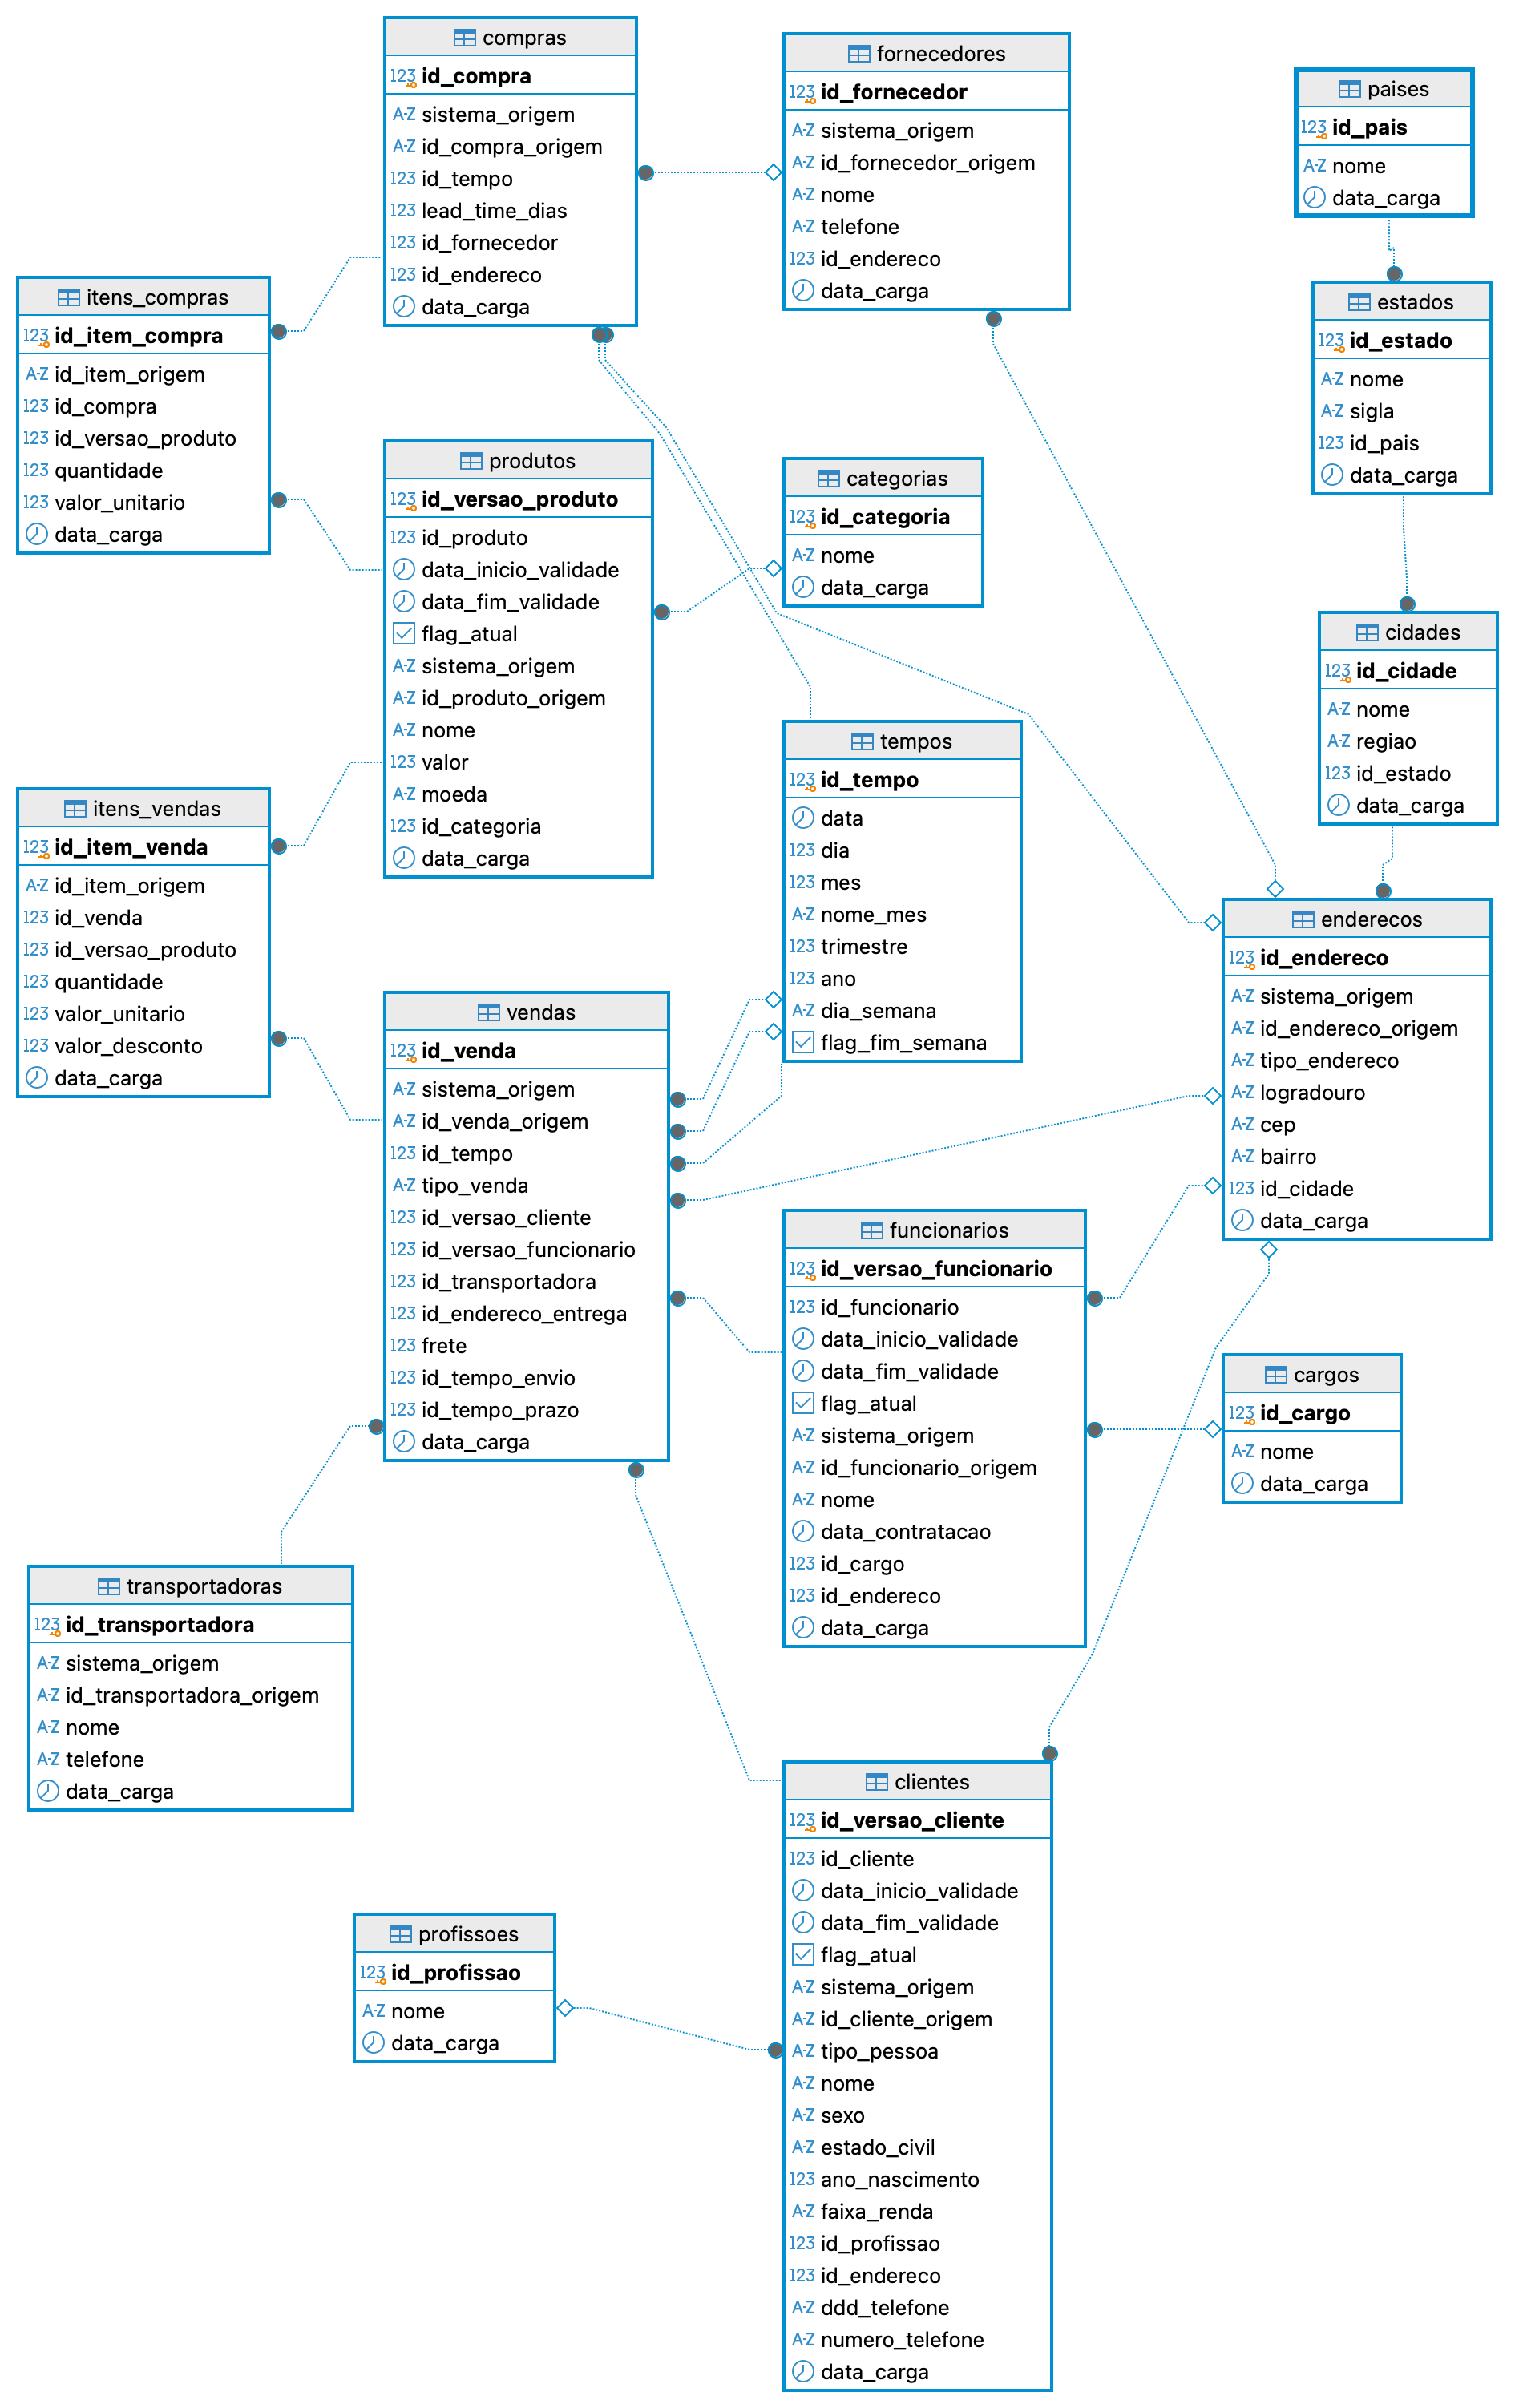
\includegraphics[width=0.8\textwidth]{./fig/dw_corporativo.png}
  \caption{Diagrama entidade-relacionamento do DW Organizacional}
  \label{fig:dw-corporativo}
  \fontefig{Elaborada pelo autor.}
\end{figure}

\begin{itemize}
    \item \textbf{Integração}: chave corporativa própria por sequência (ex.: \texttt{corporativo.seq\_clientes}) + \texttt{sistema\_origem}/id original para rastreabilidade;
    \item \textbf{Historicidade (SCD2)}: quando um atributo de cliente, funcionário ou produto muda (por exemplo, um cliente muda de faixa de renda), a linha antiga não é alterada; uma nova linha é inserida com a nova versão, e a antiga fica marcada como encerrada. Assim, o histórico completo fica preservado, e não só o valor mais recente;
    \item \textbf{Granularidade}: \texttt{vendas}/\texttt{itens\_vendas} e \texttt{compras}/\texttt{itens\_compras} têm grão de item;
    \item \textbf{Dados externos}: moeda fixa (\texttt{'BRL'}), \texttt{sistema\_origem} e membro sentinela \texttt{-1} ("Não aplicável") são atribuídos pelo ETL, documentados no catálogo de metadados (\autoref{cap:etl-bi}) como "Regras de Negócio do ETL".
\end{itemize}

DDL completo no \autoref{apend:ddl-dw}.

\chapter{Data Marts}
\label{cap:datamarts}

Três Data Marts em esquema estrela (Kimball), com arquitetura de barramento: \texttt{dim\_tempos}, \texttt{dim\_enderecos}, \texttt{dim\_produtos} e \texttt{dim\_clientes} são conformadas entre os dois sistemas; \texttt{dim\_funcionarios} e \texttt{dim\_transportadoras} usam o membro \texttt{-1} ("Não aplicável") para a Mercearia; \texttt{dim\_fornecedores} é exclusiva do Mart Compras.

\begin{figure}[H]
  \centering
  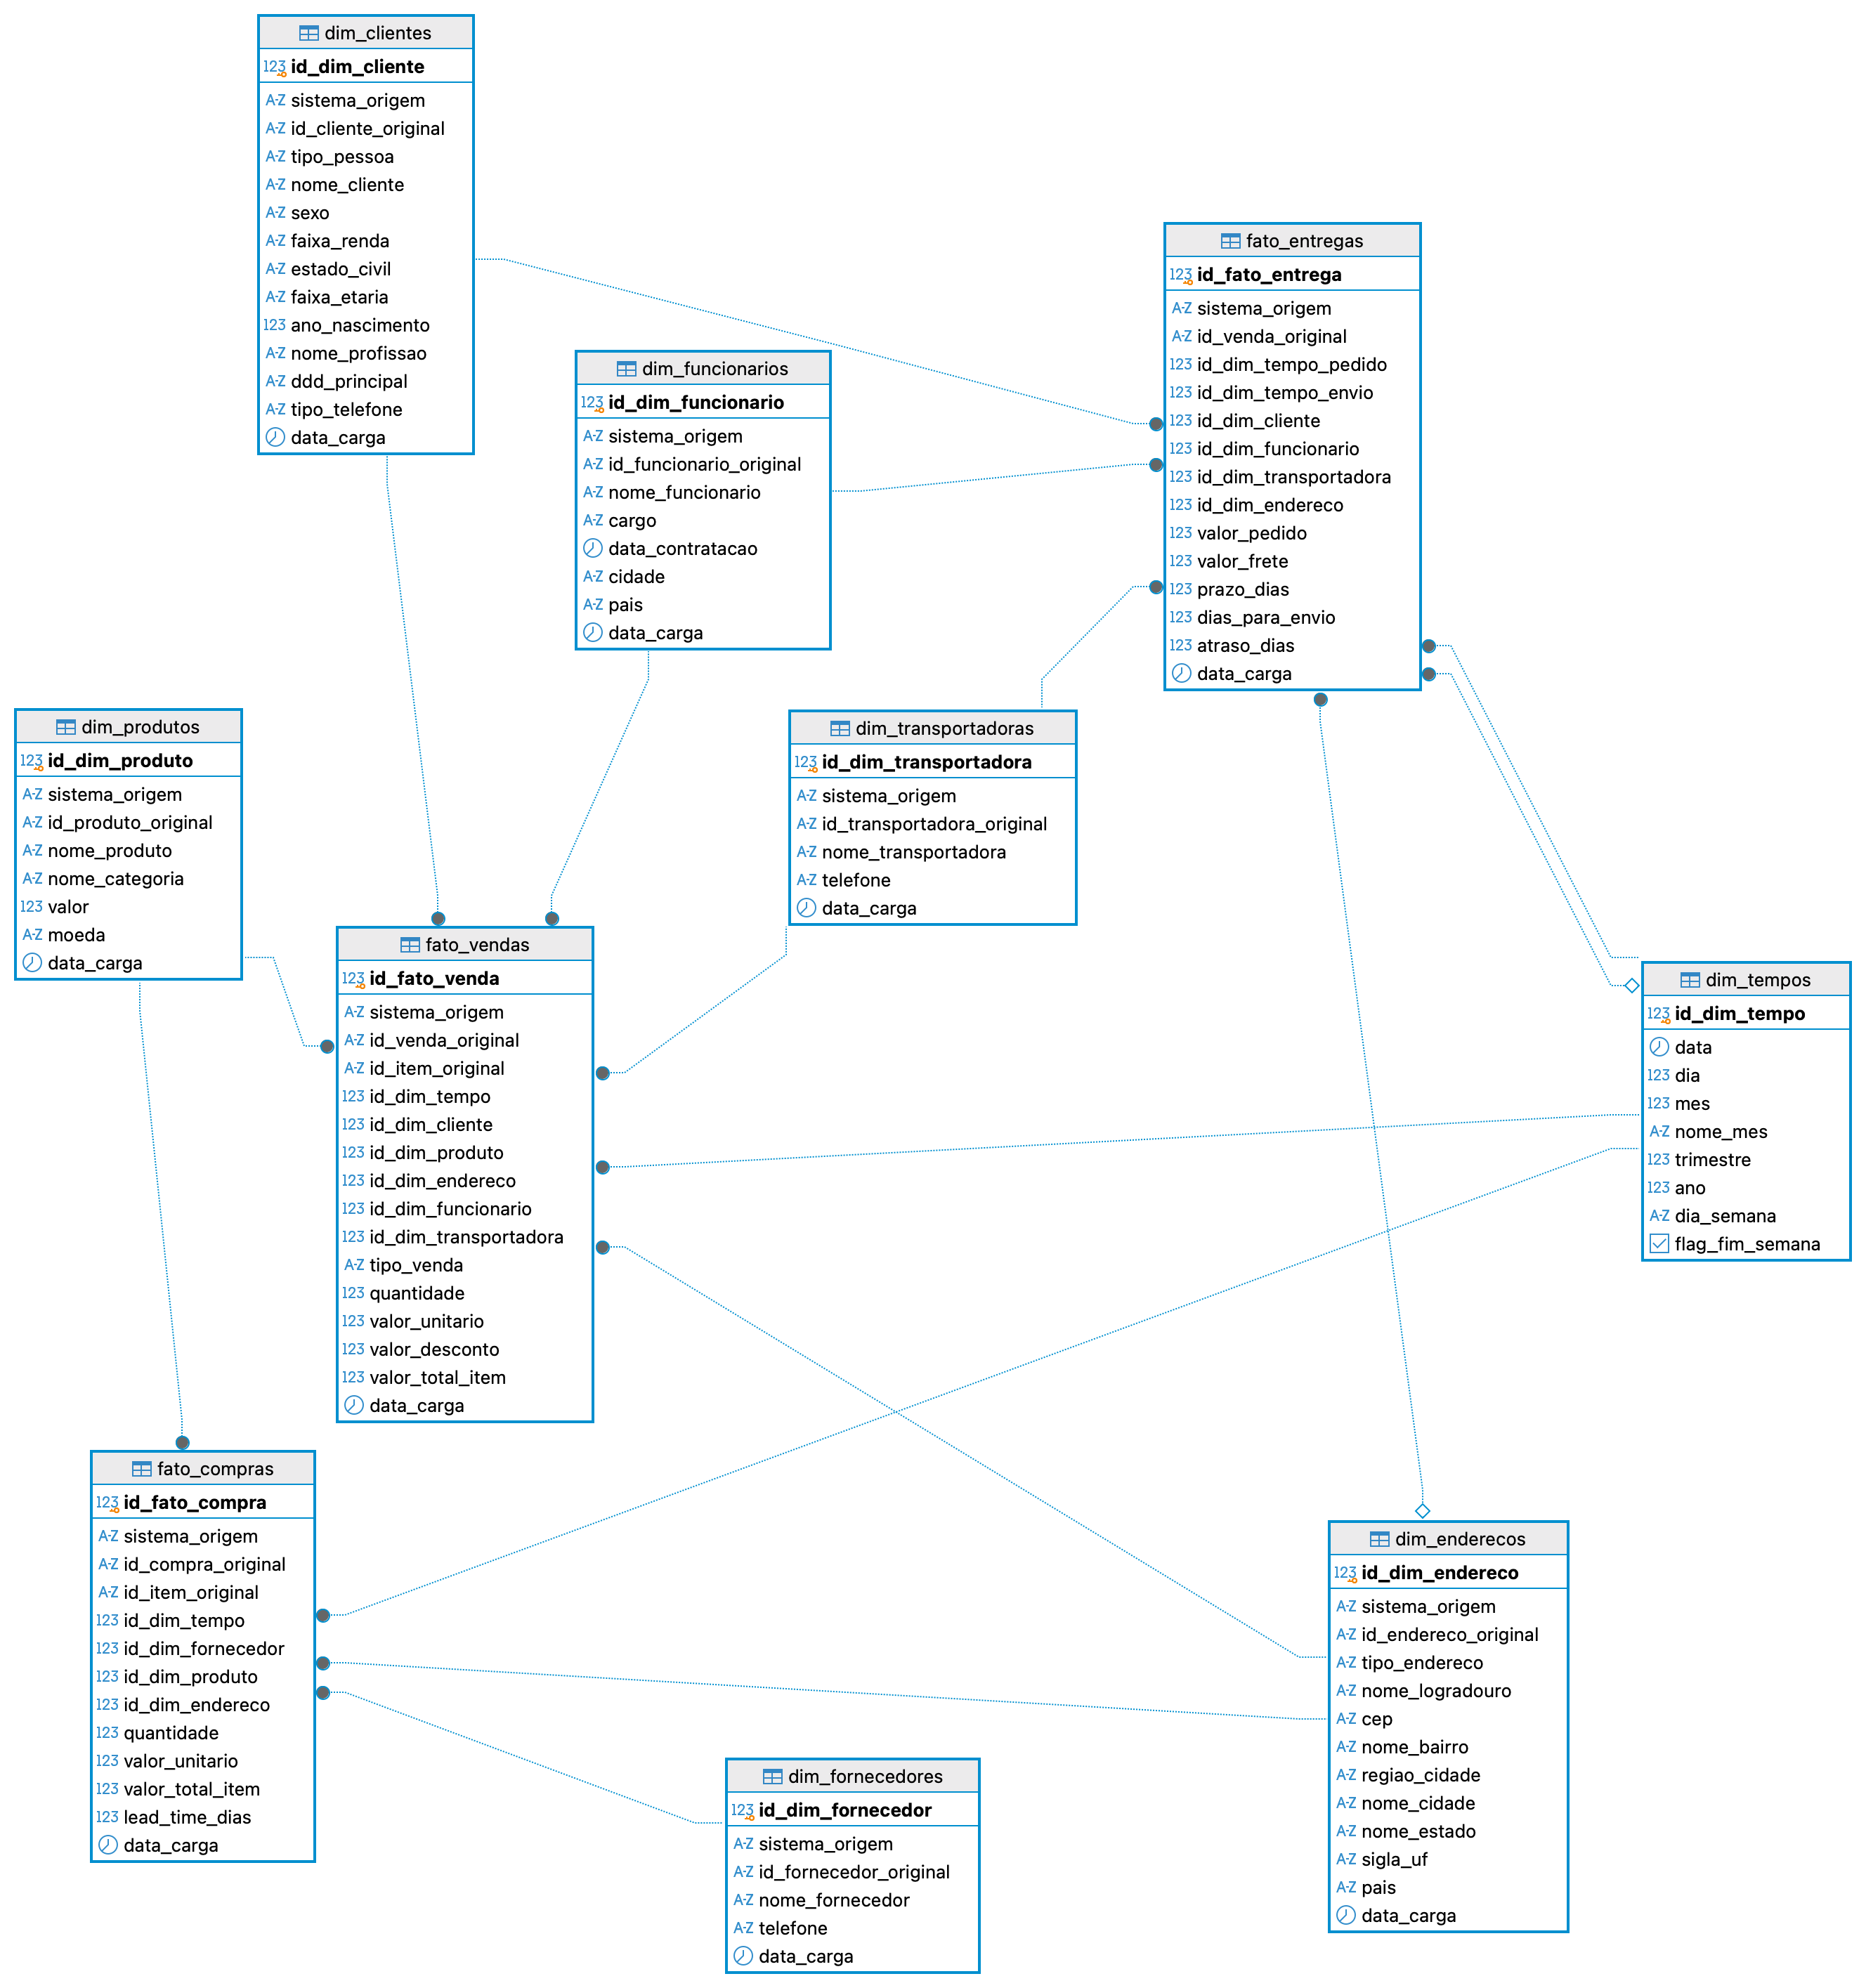
\includegraphics[width=0.8\textwidth]{./fig/dw_estrela.png}
  \caption{Diagrama entidade-relacionamento dos Data Marts}
  \label{fig:dw-estrela}
  \fontefig{Elaborada pelo autor.}
\end{figure}

\begin{quadro}[H]
\centering
\caption{Os três Data Marts: assunto, fato, grão, origem, dimensões e uso}
\label{qua:resumo-marts}
\begin{tabular}{p{1.8cm}p{2.4cm}p{1.9cm}p{3.4cm}p{4.7cm}}
\hline
\textbf{Mart} & \textbf{Fato / Grão} & \textbf{Origem} & \textbf{Dimensões} & \textbf{Uso} \\
\hline
Vendas & \texttt{fato\_vendas} (item vendido) & Northwind e Mercearia & tempo, cliente, produto, endereço, funcionário, transportadora & receita, mix de produtos, desempenho por vendedor/região \\
Compras & \texttt{fato\_compras} (item comprado) & Mercearia & tempo, fornecedor, produto, endereço & \textit{lead time}, dependência e custo de fornecedor \\
Logística e Entregas & \texttt{fato\_entregas} (pedido) & Northwind & tempo (pedido/envio), cliente, funcionário, transportadora, endereço & prazo de entrega e desempenho de transportadora, não só valor vendido \\
\hline
\end{tabular}
\fontequa{Elaborado pelo autor.}
\end{quadro}

O Mart Logística tem grão de \textbf{pedido} (não de item) de propósito, já que frete e prazo são atributos do pedido como um todo. É exclusivo do Northwind, único sistema com esse conceito, pois a Mercearia não expede fisicamente. Duas decisões de modelagem: sem conversão cambial entre moedas (campo \texttt{moeda} em \texttt{dim\_produtos}); \texttt{faixa\_renda}/\texttt{faixa\_etaria} em \texttt{dim\_clientes} são faixas descritivas, não valores brutos.

DDL completo no \autoref{apend:ddl-marts}.

\chapter{ETL, Metadados e Análise de Dados}
\label{cap:etl-bi}

\section{ETL (Apache Airflow)}
\label{sec:etl}

Duas DAGs, sempre corporativo antes de \textit{marting}:

\begin{itemize}
    \item \textbf{Carga inicial}: lê Northwind/Mercearia direto, popula o corporativo (\textit{upsert} idempotente nas tabelas de apoio) e depois os Data Marts a partir dele; fatos recriados do zero (\texttt{DELETE} + \texttt{INSERT});
    \item \textbf{Carga incremental}: usa o maior id de origem já carregado no corporativo como corte do que é novo; área de \texttt{staging} intermediária (única etapa que lê as origens); atualiza dimensões e insere só as linhas novas nos fatos, sem reler as origens.
\end{itemize}

\section{Catálogo de metadados}
\label{sec:metadados}

Esquema \texttt{metadados}: liga cada campo do DW ao seu campo transacional de origem (ou a um dado externo), com a regra de transformação aplicada. 28 tabelas / 158 campos transacionais, 10 tabelas / 109 campos do DW, 123 linhas de linhagem. DDL completo no \autoref{apend:ddl-metadados}.

\begin{figure}[H]
  \centering
  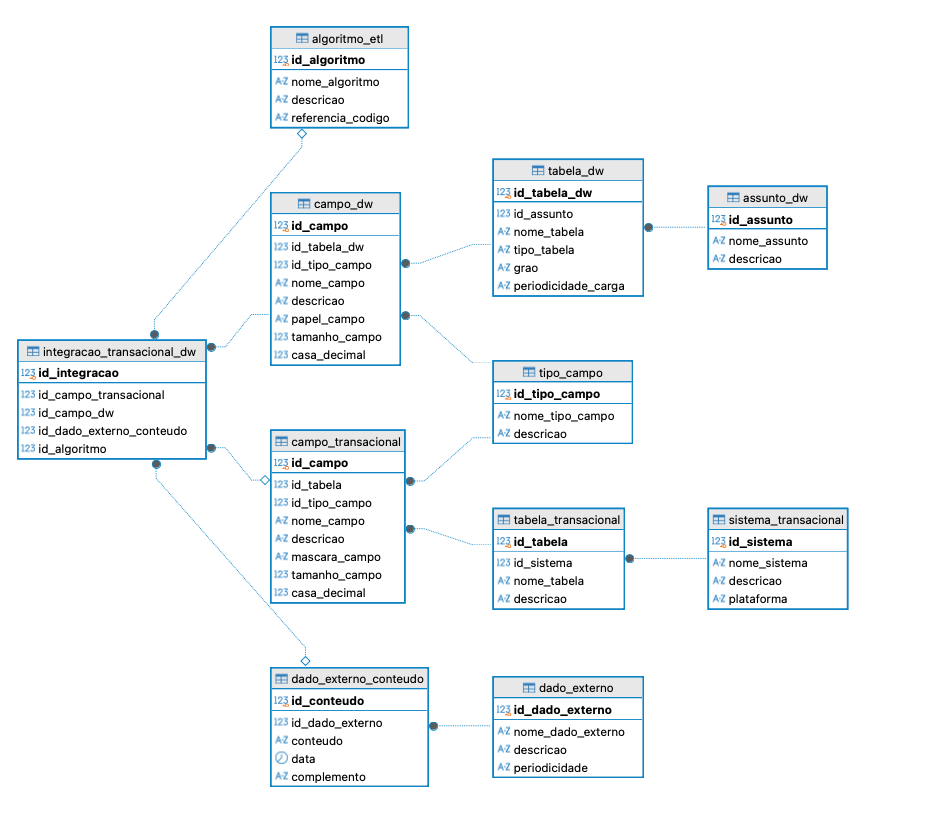
\includegraphics[width=0.9\textwidth]{./fig/metadados_modelo.png}
  \caption{Diagrama entidade-relacionamento do catálogo de metadados}
  \label{fig:metadados-modelo}
  \fontefig{Elaborada pelo autor.}
\end{figure}

\section{Business Intelligence (Metabase)}
\label{sec:bi}

Um painel por Data Mart, com consultas nativas em SQL: \textbf{Vendas} (total, ticket médio, top produtos/clientes, vendas por mês/categoria); \textbf{Compras} (\textit{lead time}, top fornecedores, compras por mês); \textbf{Logística} (prazo médio, atraso por transportadora, \% no prazo).

\begin{figure}[H]
  \centering
  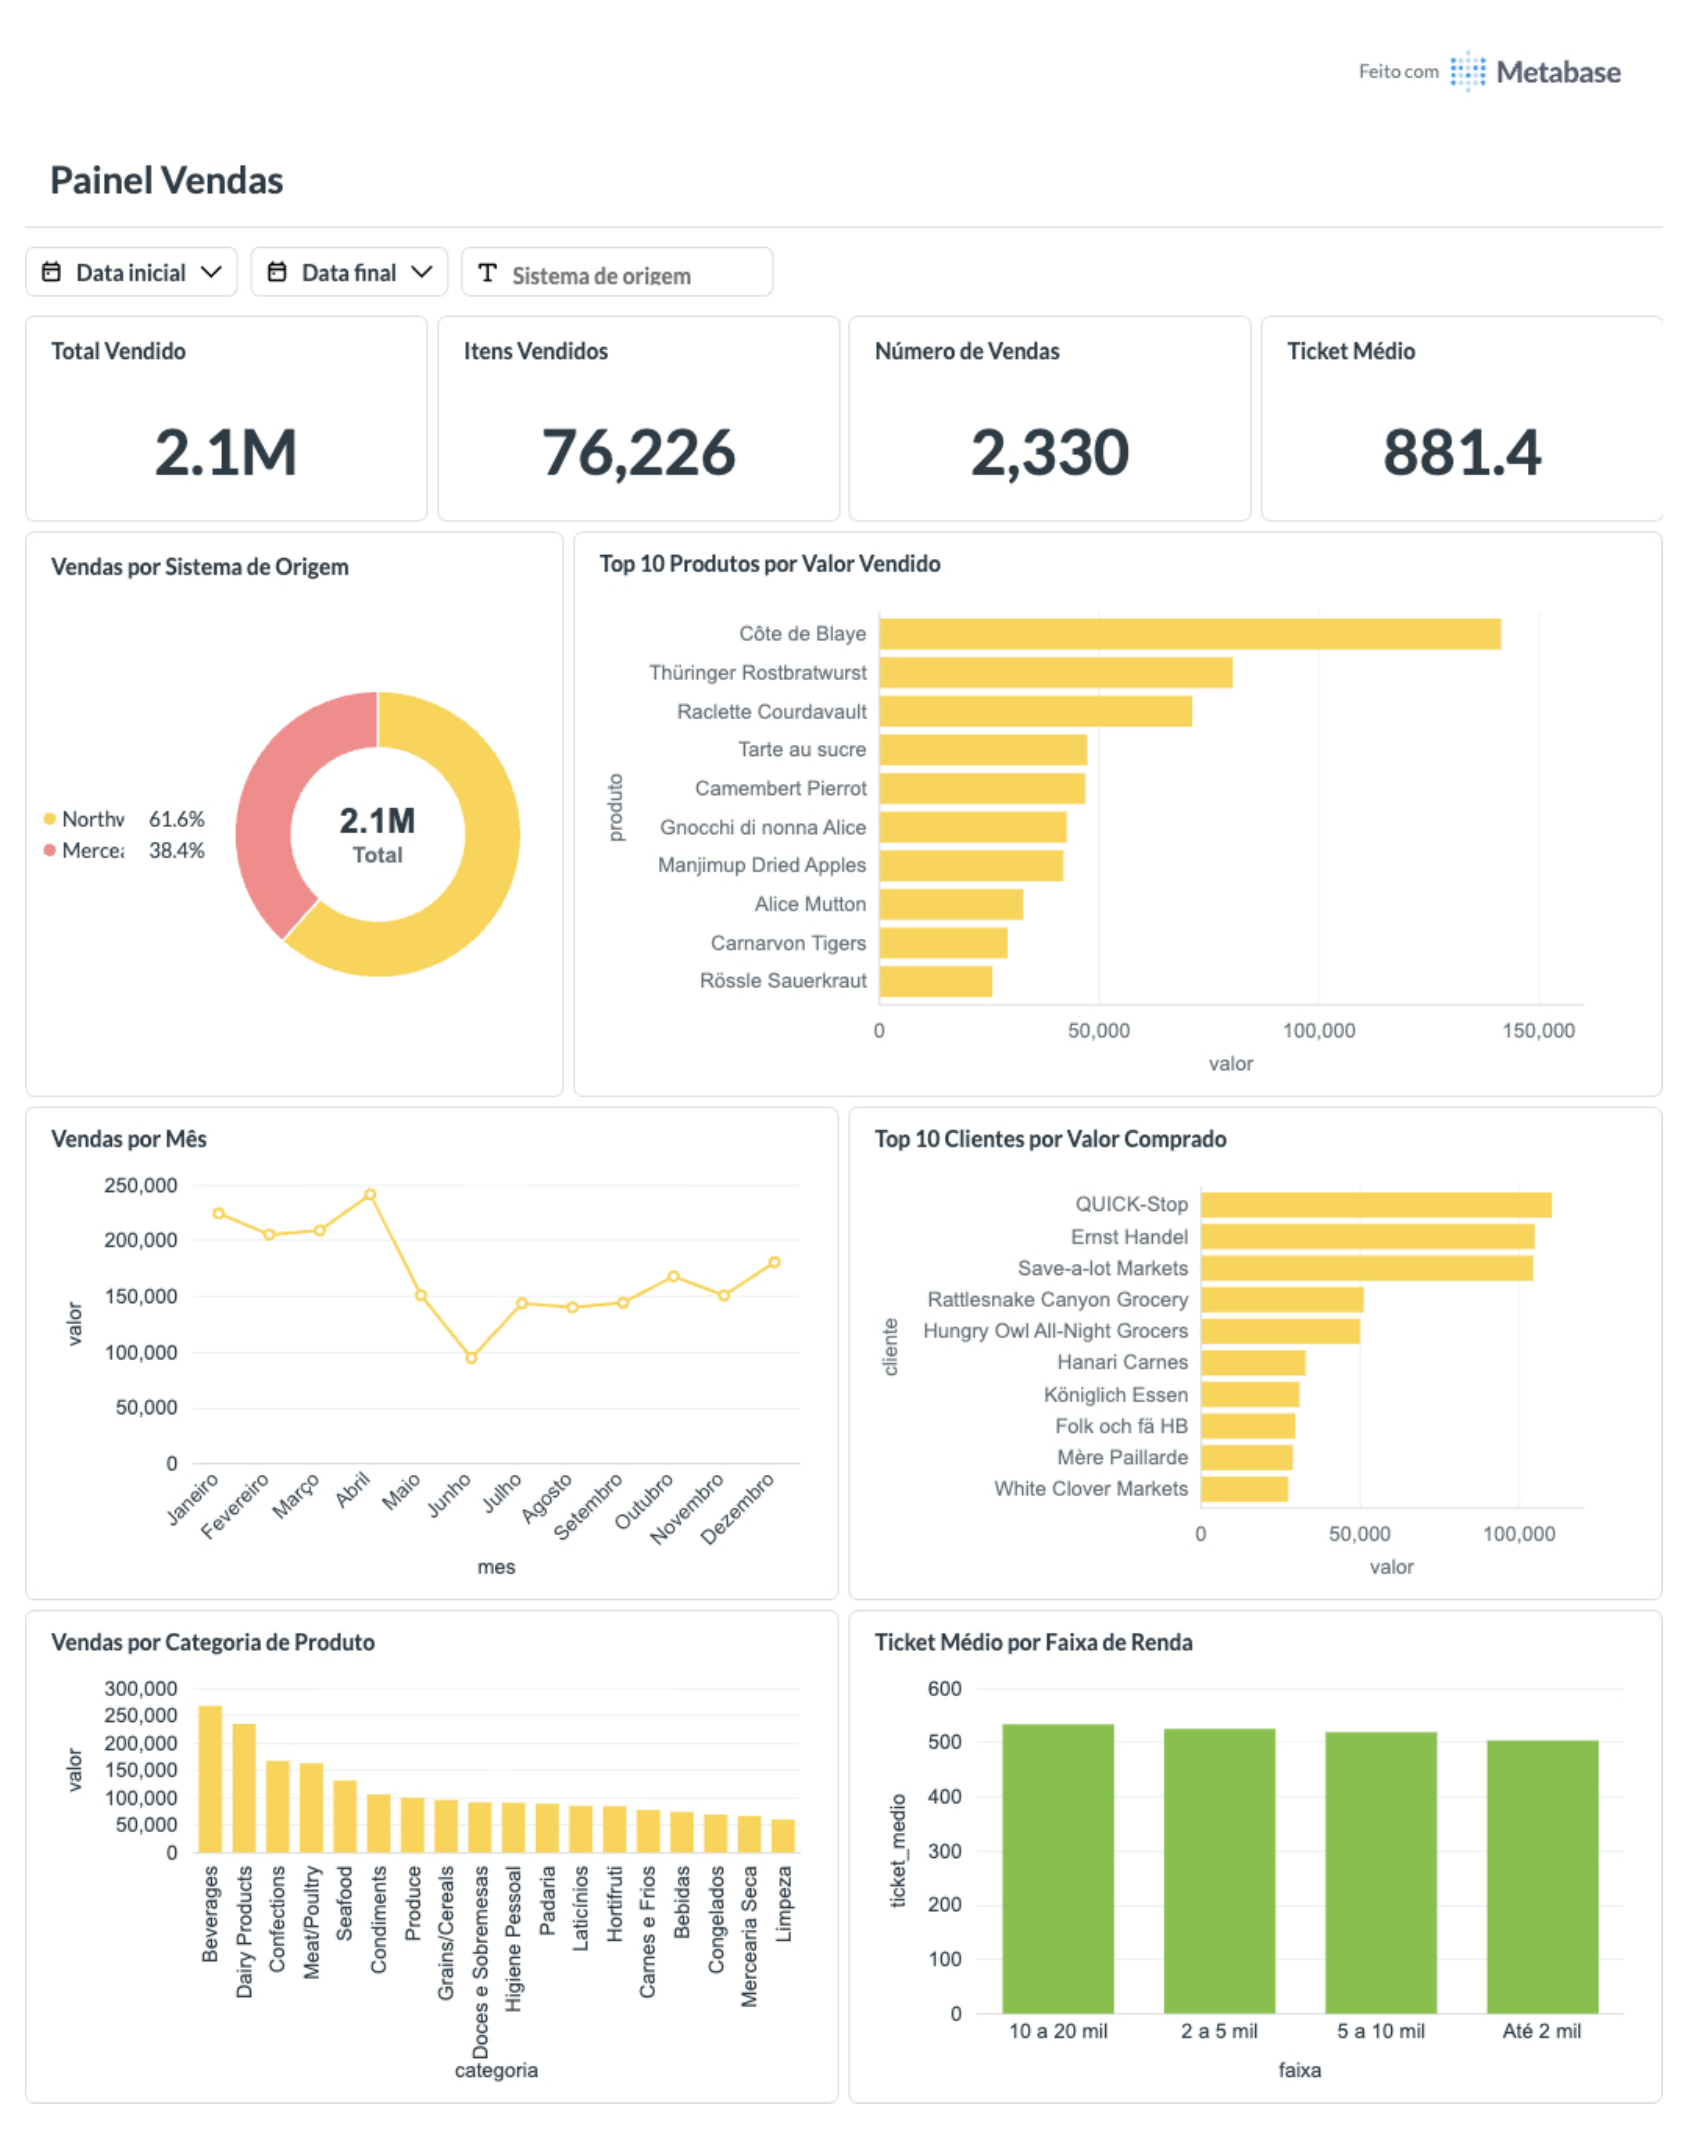
\includegraphics[width=0.75\textwidth]{./fig/dashboard_vendas_preview.png}
  \caption{Painel Vendas no Metabase}
  \label{fig:dashboard-vendas}
  \fontefig{Elaborada pelo autor, a partir do Metabase.}
\end{figure}

\chapter{Conclusão}
\label{cap:conclusao}

O DW Organizacional foi construído integrando Northwind e Mercearia, com os três Data Marts (Vendas, Compras e Logística) derivados dele, carga via Airflow e o catálogo de metadados documentando a origem de cada campo. Os painéis no Metabase mostram que o modelo responde às perguntas de negócio propostas para cada Data Mart. Como próximo passo, a carga incremental poderia rodar em um agendamento automático, em vez de disparada manualmente.

Uma dificuldade do processo foi conciliar o código do ETL com o catálogo de metadados: como a lógica de carga está \textit{hard-coded} nas DAGs do Airflow, cada regra de transformação precisou ser descrita manualmente na tabela \texttt{algoritmo\_etl}, em vez de o catálogo ser gerado a partir do próprio código.




% NÃO EDITAR ------------------------------------------------------ %
\bibliografia



% EDITAR - Todos os cursos ---------------------------------------- %
% Use o trecho abaixo para inserir apêndices e anexos usando o
% comando input da mesma forma que para capítulos. NÃO edite nem
% altere a ordem dos comandos \apendices e \anexos.
% Se não houver apêndice e anexo remova os comandos input
% equivalentes
% ---- Apêndices
\apendices
\chapter{DDL do Data Warehouse Organizacional}
\label{apend:ddl-dw}

DDL completo do esquema \texttt{corporativo} (DW Organizacional, \autoref{cap:dw-organizacional}). Também no repositório do projeto, em \texttt{application/dw/dw\_postgres.sql}.

{\footnotesize
\begin{verbatim}
CREATE DATABASE dw;

\c dw

CREATE SCHEMA corporativo;

-- ----------------------------
-- ASSUNTO: TEMPO
-- ----------------------------
-- Calendario corporativo, gerado uma vez (nao vem de sistema
-- transacional). Compartilhado por todos os assuntos, igual a
-- Geografia, por isso fica antes dos demais.

CREATE TABLE corporativo.tempos (
    id_tempo INT GENERATED BY DEFAULT AS IDENTITY PRIMARY KEY,
    data DATE NOT NULL,
    dia INT NOT NULL,
    mes INT NOT NULL,
    nome_mes VARCHAR(20) NOT NULL,
    trimestre INT NOT NULL,
    ano INT NOT NULL,
    dia_semana VARCHAR(20) NOT NULL,
    flag_fim_semana BOOLEAN NOT NULL,
    UNIQUE (data)
);

INSERT INTO corporativo.tempos
    (data, dia, mes, nome_mes, trimestre, ano, dia_semana, flag_fim_semana)
SELECT
    d::date,
    EXTRACT(DAY FROM d)::int,
    EXTRACT(MONTH FROM d)::int,
    TO_CHAR(d, 'TMMonth'),
    EXTRACT(QUARTER FROM d)::int,
    EXTRACT(YEAR FROM d)::int,
    TO_CHAR(d, 'TMDay'),
    EXTRACT(ISODOW FROM d) IN (6, 7)
FROM generate_series('1996-01-01'::date, '2035-12-31'::date, interval '1 day') AS d;

-- ----------------------------
-- ASSUNTO: GEOGRAFIA
-- ----------------------------

CREATE TABLE corporativo.paises (
    id_pais INT GENERATED BY DEFAULT AS IDENTITY PRIMARY KEY,
    nome VARCHAR(100) NOT NULL,
    data_carga TIMESTAMP NOT NULL DEFAULT now(),
    UNIQUE (nome)
);

CREATE TABLE corporativo.estados (
    id_estado INT GENERATED BY DEFAULT AS IDENTITY PRIMARY KEY,
    nome VARCHAR(100) NOT NULL,
    sigla VARCHAR(10) NOT NULL,
    id_pais INT NOT NULL REFERENCES corporativo.paises (id_pais),
    data_carga TIMESTAMP NOT NULL DEFAULT now(),
    UNIQUE (id_pais, sigla)
);

CREATE TABLE corporativo.cidades (
    id_cidade INT GENERATED BY DEFAULT AS IDENTITY PRIMARY KEY,
    nome VARCHAR(255) NOT NULL,
    regiao VARCHAR(255),
    id_estado INT NOT NULL REFERENCES corporativo.estados (id_estado),
    data_carga TIMESTAMP NOT NULL DEFAULT now(),
    UNIQUE (id_estado, nome)
);

CREATE TABLE corporativo.enderecos (
    id_endereco INT GENERATED BY DEFAULT AS IDENTITY PRIMARY KEY,
    sistema_origem VARCHAR(20) NOT NULL,
    id_endereco_origem VARCHAR(50),
    tipo_endereco VARCHAR(45),
    logradouro VARCHAR(255),
    cep VARCHAR(20),
    bairro VARCHAR(255),
    id_cidade INT NOT NULL REFERENCES corporativo.cidades (id_cidade),
    data_carga TIMESTAMP NOT NULL DEFAULT now(),
    UNIQUE (sistema_origem, id_endereco_origem)
);

-- ----------------------------
-- ASSUNTO: PESSOAS
-- ----------------------------

CREATE TABLE corporativo.profissoes (
    id_profissao INT GENERATED BY DEFAULT AS IDENTITY PRIMARY KEY,
    nome VARCHAR(255) NOT NULL,
    data_carga TIMESTAMP NOT NULL DEFAULT now(),
    UNIQUE (nome)
);

CREATE SEQUENCE corporativo.seq_clientes START 1;

-- id_versao_cliente e a PK real (uma linha = uma versao do cliente);
-- id_cliente e a identidade estavel entre versoes (nao muda num SCD2).
CREATE TABLE corporativo.clientes (
    id_versao_cliente BIGINT GENERATED BY DEFAULT AS IDENTITY PRIMARY KEY,
    id_cliente INT NOT NULL DEFAULT nextval('corporativo.seq_clientes'),
    data_inicio_validade DATE NOT NULL DEFAULT CURRENT_DATE,
    data_fim_validade DATE,
    flag_atual BOOLEAN NOT NULL DEFAULT TRUE,
    sistema_origem VARCHAR(20) NOT NULL,
    id_cliente_origem VARCHAR(50) NOT NULL,
    tipo_pessoa VARCHAR(20) NOT NULL,
    nome VARCHAR(255) NOT NULL,
    sexo VARCHAR(20),
    estado_civil VARCHAR(45),
    ano_nascimento INT,
    faixa_renda VARCHAR(50),
    id_profissao INT REFERENCES corporativo.profissoes (id_profissao),
    id_endereco INT REFERENCES corporativo.enderecos (id_endereco),
    ddd_telefone VARCHAR(10),
    numero_telefone VARCHAR(20),
    data_carga TIMESTAMP NOT NULL DEFAULT now(),
    UNIQUE (sistema_origem, id_cliente_origem, data_inicio_validade)
);

CREATE TABLE corporativo.cargos (
    id_cargo INT GENERATED BY DEFAULT AS IDENTITY PRIMARY KEY,
    nome VARCHAR(255) NOT NULL,
    data_carga TIMESTAMP NOT NULL DEFAULT now(),
    UNIQUE (nome)
);

CREATE SEQUENCE corporativo.seq_funcionarios START 1;

-- id_versao_funcionario e a PK real, mesma logica de clientes acima.
CREATE TABLE corporativo.funcionarios (
    id_versao_funcionario BIGINT GENERATED BY DEFAULT AS IDENTITY PRIMARY KEY,
    id_funcionario INT NOT NULL DEFAULT nextval('corporativo.seq_funcionarios'),
    data_inicio_validade DATE NOT NULL DEFAULT CURRENT_DATE,
    data_fim_validade DATE,
    flag_atual BOOLEAN NOT NULL DEFAULT TRUE,
    sistema_origem VARCHAR(20) NOT NULL,
    id_funcionario_origem VARCHAR(50),
    nome VARCHAR(255) NOT NULL,
    data_contratacao DATE,
    id_cargo INT REFERENCES corporativo.cargos (id_cargo),
    id_endereco INT REFERENCES corporativo.enderecos (id_endereco),
    data_carga TIMESTAMP NOT NULL DEFAULT now(),
    UNIQUE (sistema_origem, id_funcionario_origem, data_inicio_validade)
);

-- Sentinela "Nao aplicavel": id_versao_funcionario tambem fixado em -1 (em
-- vez de deixar a IDENTITY gerar), pra vendas.id_versao_funcionario poder
-- usar DEFAULT -1 apontando pra essa mesma linha via FK de verdade.
INSERT INTO corporativo.funcionarios
    (id_versao_funcionario, id_funcionario, sistema_origem,
     id_funcionario_origem, nome)
VALUES (-1, -1, 'N/A', NULL, 'Nao aplicavel');

-- ----------------------------
-- ASSUNTO: PRODUTO E PARCEIROS
-- ----------------------------

CREATE TABLE corporativo.categorias (
    id_categoria INT GENERATED BY DEFAULT AS IDENTITY PRIMARY KEY,
    nome VARCHAR(255) NOT NULL,
    data_carga TIMESTAMP NOT NULL DEFAULT now(),
    UNIQUE (nome)
);

CREATE SEQUENCE corporativo.seq_produtos START 1;

-- id_versao_produto e a PK real, mesma logica de clientes/funcionarios.
CREATE TABLE corporativo.produtos (
    id_versao_produto BIGINT GENERATED BY DEFAULT AS IDENTITY PRIMARY KEY,
    id_produto INT NOT NULL DEFAULT nextval('corporativo.seq_produtos'),
    data_inicio_validade DATE NOT NULL DEFAULT CURRENT_DATE,
    data_fim_validade DATE,
    flag_atual BOOLEAN NOT NULL DEFAULT TRUE,
    sistema_origem VARCHAR(20) NOT NULL,
    id_produto_origem VARCHAR(50) NOT NULL,
    nome VARCHAR(255) NOT NULL,
    valor NUMERIC(15,2),
    moeda CHAR(3) NOT NULL DEFAULT 'BRL',
    id_categoria INT REFERENCES corporativo.categorias (id_categoria),
    data_carga TIMESTAMP NOT NULL DEFAULT now(),
    UNIQUE (sistema_origem, id_produto_origem, data_inicio_validade)
);

CREATE TABLE corporativo.transportadoras (
    id_transportadora INT GENERATED BY DEFAULT AS IDENTITY PRIMARY KEY,
    sistema_origem VARCHAR(20) NOT NULL,
    id_transportadora_origem VARCHAR(50),
    nome VARCHAR(255) NOT NULL,
    telefone VARCHAR(50),
    data_carga TIMESTAMP NOT NULL DEFAULT now(),
    UNIQUE (sistema_origem, id_transportadora_origem)
);

INSERT INTO corporativo.transportadoras
    (id_transportadora, sistema_origem, id_transportadora_origem, nome)
VALUES (-1, 'N/A', NULL, 'Nao aplicavel');

CREATE TABLE corporativo.fornecedores (
    id_fornecedor INT GENERATED BY DEFAULT AS IDENTITY PRIMARY KEY,
    sistema_origem VARCHAR(20) NOT NULL,
    id_fornecedor_origem VARCHAR(50),
    nome VARCHAR(255) NOT NULL,
    telefone VARCHAR(50),
    id_endereco INT REFERENCES corporativo.enderecos (id_endereco),
    data_carga TIMESTAMP NOT NULL DEFAULT now(),
    UNIQUE (sistema_origem, id_fornecedor_origem)
);

-- ----------------------------
-- ASSUNTO: TRANSACOES
-- ----------------------------

CREATE TABLE corporativo.vendas (
    id_venda BIGINT GENERATED BY DEFAULT AS IDENTITY PRIMARY KEY,
    sistema_origem VARCHAR(20) NOT NULL,
    id_venda_origem VARCHAR(50) NOT NULL,
    id_tempo INT NOT NULL REFERENCES corporativo.tempos (id_tempo),
    tipo_venda VARCHAR(50),
    -- Aponta pra versao do cliente/funcionario vigente no momento da venda,
    -- resolvida pelo ETL na carga (nao em tempo de consulta): por isso e
    -- uma FK de verdade, e nao uma juncao temporal contra id_cliente/
    -- id_funcionario (que so identificam a entidade, nao a versao).
    id_versao_cliente BIGINT NOT NULL
        REFERENCES corporativo.clientes (id_versao_cliente),
    id_versao_funcionario BIGINT NOT NULL DEFAULT -1
        REFERENCES corporativo.funcionarios (id_versao_funcionario),
    id_transportadora INT NOT NULL DEFAULT -1
        REFERENCES corporativo.transportadoras (id_transportadora),
    id_endereco_entrega INT REFERENCES corporativo.enderecos (id_endereco),
    frete NUMERIC(15,2), -- exclusivo do Northwind (orders.freight)
    id_tempo_envio INT REFERENCES corporativo.tempos (id_tempo), -- Northwind
    id_tempo_prazo INT REFERENCES corporativo.tempos (id_tempo), -- Northwind
    data_carga TIMESTAMP NOT NULL DEFAULT now(),
    UNIQUE (sistema_origem, id_venda_origem)
);

CREATE INDEX idx_venda_cliente ON corporativo.vendas (id_versao_cliente);
CREATE INDEX idx_venda_funcionario ON corporativo.vendas (id_versao_funcionario);
CREATE INDEX idx_venda_tempo ON corporativo.vendas (id_tempo);

CREATE TABLE corporativo.itens_vendas (
    id_item_venda BIGINT GENERATED BY DEFAULT AS IDENTITY PRIMARY KEY,
    id_item_origem VARCHAR(50),
    id_venda BIGINT NOT NULL REFERENCES corporativo.vendas (id_venda),
    -- Versao do produto vigente na data da venda, resolvida pelo ETL.
    id_versao_produto BIGINT NOT NULL
        REFERENCES corporativo.produtos (id_versao_produto),
    quantidade INT NOT NULL,
    valor_unitario NUMERIC(15,2) NOT NULL,
    valor_desconto NUMERIC(15,2) NOT NULL DEFAULT 0,
    data_carga TIMESTAMP NOT NULL DEFAULT now()
);

CREATE INDEX idx_item_venda_venda ON corporativo.itens_vendas (id_venda);
CREATE INDEX idx_item_venda_produto ON corporativo.itens_vendas (id_versao_produto);

CREATE TABLE corporativo.compras (
    id_compra BIGINT GENERATED BY DEFAULT AS IDENTITY PRIMARY KEY,
    sistema_origem VARCHAR(20) NOT NULL DEFAULT 'Mercearia',
    id_compra_origem VARCHAR(50) NOT NULL,
    id_tempo INT NOT NULL REFERENCES corporativo.tempos (id_tempo),
    lead_time_dias INT,
    id_fornecedor INT REFERENCES corporativo.fornecedores (id_fornecedor),
    id_endereco INT REFERENCES corporativo.enderecos (id_endereco),
    data_carga TIMESTAMP NOT NULL DEFAULT now(),
    UNIQUE (sistema_origem, id_compra_origem)
);

CREATE INDEX idx_compra_fornecedor ON corporativo.compras (id_fornecedor);
CREATE INDEX idx_compra_tempo ON corporativo.compras (id_tempo);

CREATE TABLE corporativo.itens_compras (
    id_item_compra BIGINT GENERATED BY DEFAULT AS IDENTITY PRIMARY KEY,
    id_item_origem VARCHAR(50),
    id_compra BIGINT NOT NULL REFERENCES corporativo.compras (id_compra),
    id_versao_produto BIGINT NOT NULL
        REFERENCES corporativo.produtos (id_versao_produto),
    quantidade INT NOT NULL,
    valor_unitario NUMERIC(15,2) NOT NULL,
    data_carga TIMESTAMP NOT NULL DEFAULT now()
);

CREATE INDEX idx_item_compra_compra ON corporativo.itens_compras (id_compra);
CREATE INDEX idx_item_compra_produto ON corporativo.itens_compras (id_versao_produto);
\end{verbatim}
}

\chapter{DDL dos Data Marts}
\label{apend:ddl-marts}

DDL completo do esquema estrela dos três Data Marts (\autoref{cap:datamarts}): dimensões conformadas, fatos e a geração da \texttt{dim\_tempos}. Também no repositório do projeto, em \texttt{application/data\_marting/}.

{\footnotesize
\begin{verbatim}
\c dw

-- ----------------------------
-- DIMENSOES
-- ----------------------------

CREATE TABLE dim_tempos (
    id_dim_tempo INT GENERATED BY DEFAULT AS IDENTITY PRIMARY KEY,
    data DATE NOT NULL,
    dia INT NOT NULL,
    mes INT NOT NULL,
    nome_mes VARCHAR(20) NOT NULL,
    trimestre INT NOT NULL,
    ano INT NOT NULL,
    dia_semana VARCHAR(20) NOT NULL,
    flag_fim_semana BOOLEAN NOT NULL,
    UNIQUE (data)
);

CREATE TABLE dim_enderecos (
    id_dim_endereco INT GENERATED BY DEFAULT AS IDENTITY PRIMARY KEY,
    sistema_origem VARCHAR(20) NOT NULL,
    id_endereco_original VARCHAR(50),
    tipo_endereco VARCHAR(45),
    nome_logradouro VARCHAR(255),
    cep VARCHAR(20),
    nome_bairro VARCHAR(255),
    regiao_cidade VARCHAR(255),
    nome_cidade VARCHAR(255),
    nome_estado VARCHAR(100),
    sigla_uf VARCHAR(10),
    pais VARCHAR(100) NOT NULL,
    data_carga TIMESTAMP NOT NULL DEFAULT now(),
    UNIQUE (sistema_origem, id_endereco_original)
);

CREATE TABLE dim_produtos (
    id_dim_produto INT GENERATED BY DEFAULT AS IDENTITY PRIMARY KEY,
    sistema_origem VARCHAR(20) NOT NULL,
    id_produto_original VARCHAR(50) NOT NULL,
    nome_produto VARCHAR(255) NOT NULL,
    nome_categoria VARCHAR(255),
    valor NUMERIC(15,2),
    moeda CHAR(3) NOT NULL DEFAULT 'BRL',
    data_carga TIMESTAMP NOT NULL DEFAULT now(),
    UNIQUE (sistema_origem, id_produto_original)
);

CREATE TABLE dim_clientes (
    id_dim_cliente INT GENERATED BY DEFAULT AS IDENTITY PRIMARY KEY,
    sistema_origem VARCHAR(20) NOT NULL,
    id_cliente_original VARCHAR(50) NOT NULL,
    tipo_pessoa VARCHAR(20) NOT NULL,
    nome_cliente VARCHAR(255) NOT NULL,
    sexo VARCHAR(20),
    faixa_renda VARCHAR(50),
    estado_civil VARCHAR(45),
    faixa_etaria VARCHAR(20),
    ano_nascimento INT,
    nome_profissao VARCHAR(255),
    ddd_principal VARCHAR(10),
    tipo_telefone VARCHAR(50),
    data_carga TIMESTAMP NOT NULL DEFAULT now(),
    UNIQUE (sistema_origem, id_cliente_original)
);

CREATE TABLE dim_funcionarios (
    id_dim_funcionario INT GENERATED BY DEFAULT AS IDENTITY PRIMARY KEY,
    sistema_origem VARCHAR(20) NOT NULL,
    id_funcionario_original VARCHAR(50),
    nome_funcionario VARCHAR(255) NOT NULL,
    cargo VARCHAR(255),
    data_contratacao DATE,
    cidade VARCHAR(255),
    pais VARCHAR(100),
    data_carga TIMESTAMP NOT NULL DEFAULT now(),
    UNIQUE (sistema_origem, id_funcionario_original)
);

INSERT INTO dim_funcionarios
    (id_dim_funcionario, sistema_origem, id_funcionario_original,
     nome_funcionario, cargo)
VALUES (-1, 'N/A', NULL, 'Nao aplicavel', 'Nao aplicavel');

CREATE TABLE dim_transportadoras (
    id_dim_transportadora INT GENERATED BY DEFAULT AS IDENTITY PRIMARY KEY,
    sistema_origem VARCHAR(20) NOT NULL,
    id_transportadora_original VARCHAR(50),
    nome_transportadora VARCHAR(255) NOT NULL,
    telefone VARCHAR(50),
    data_carga TIMESTAMP NOT NULL DEFAULT now(),
    UNIQUE (sistema_origem, id_transportadora_original)
);

INSERT INTO dim_transportadoras
    (id_dim_transportadora, sistema_origem, id_transportadora_original,
     nome_transportadora)
VALUES (-1, 'N/A', NULL, 'Nao aplicavel');

CREATE TABLE dim_fornecedores (
    id_dim_fornecedor INT GENERATED BY DEFAULT AS IDENTITY PRIMARY KEY,
    sistema_origem VARCHAR(20) NOT NULL,
    id_fornecedor_original VARCHAR(50),
    nome_fornecedor VARCHAR(255) NOT NULL,
    telefone VARCHAR(50),
    data_carga TIMESTAMP NOT NULL DEFAULT now(),
    UNIQUE (sistema_origem, id_fornecedor_original)
);

-- ----------------------------
-- FATOS
-- ----------------------------

CREATE TABLE fato_vendas (
    id_fato_venda BIGINT GENERATED BY DEFAULT AS IDENTITY PRIMARY KEY,
    sistema_origem VARCHAR(20) NOT NULL,
    id_venda_original VARCHAR(50) NOT NULL,
    id_item_original VARCHAR(50),
    id_dim_tempo INT NOT NULL REFERENCES dim_tempos (id_dim_tempo),
    id_dim_cliente INT NOT NULL REFERENCES dim_clientes (id_dim_cliente),
    id_dim_produto INT NOT NULL REFERENCES dim_produtos (id_dim_produto),
    id_dim_endereco INT NOT NULL REFERENCES dim_enderecos (id_dim_endereco),
    id_dim_funcionario INT NOT NULL DEFAULT -1
        REFERENCES dim_funcionarios (id_dim_funcionario),
    id_dim_transportadora INT NOT NULL DEFAULT -1
        REFERENCES dim_transportadoras (id_dim_transportadora),
    tipo_venda VARCHAR(50),
    quantidade INT NOT NULL,
    valor_unitario NUMERIC(15,2) NOT NULL,
    valor_desconto NUMERIC(15,2) NOT NULL DEFAULT 0,
    valor_total_item NUMERIC(15,2) NOT NULL,
    data_carga TIMESTAMP NOT NULL DEFAULT now()
);

CREATE INDEX idx_fato_vendas_tempo ON fato_vendas (id_dim_tempo);
CREATE INDEX idx_fato_vendas_cliente ON fato_vendas (id_dim_cliente);
CREATE INDEX idx_fato_vendas_produto ON fato_vendas (id_dim_produto);
CREATE INDEX idx_fato_vendas_endereco ON fato_vendas (id_dim_endereco);
CREATE INDEX idx_fato_vendas_funcionario ON fato_vendas (id_dim_funcionario);
CREATE INDEX idx_fato_vendas_transportadora ON fato_vendas (id_dim_transportadora);

CREATE TABLE fato_compras (
    id_fato_compra BIGINT GENERATED BY DEFAULT AS IDENTITY PRIMARY KEY,
    sistema_origem VARCHAR(20) NOT NULL DEFAULT 'Mercearia',
    id_compra_original VARCHAR(50) NOT NULL,
    id_item_original VARCHAR(50),
    id_dim_tempo INT NOT NULL REFERENCES dim_tempos (id_dim_tempo),
    id_dim_fornecedor INT NOT NULL REFERENCES dim_fornecedores (id_dim_fornecedor),
    id_dim_produto INT NOT NULL REFERENCES dim_produtos (id_dim_produto),
    id_dim_endereco INT NOT NULL REFERENCES dim_enderecos (id_dim_endereco),
    quantidade INT NOT NULL,
    valor_unitario NUMERIC(15,2) NOT NULL,
    valor_total_item NUMERIC(15,2) NOT NULL,
    lead_time_dias INT,
    data_carga TIMESTAMP NOT NULL DEFAULT now()
);

CREATE INDEX idx_fato_compras_tempo ON fato_compras (id_dim_tempo);
CREATE INDEX idx_fato_compras_fornecedor ON fato_compras (id_dim_fornecedor);
CREATE INDEX idx_fato_compras_produto ON fato_compras (id_dim_produto);
CREATE INDEX idx_fato_compras_endereco ON fato_compras (id_dim_endereco);

-- Mart Logistica/Entregas: grao de 1 linha por pedido (cabecalho da venda,
-- nao por item). Exclusivo do Northwind, unico sistema de origem com o
-- conceito de frete/prazo/data de envio; reaproveita as dimensoes
-- conformadas ja existentes em vez de duplica-las.
CREATE TABLE fato_entregas (
    id_fato_entrega BIGINT GENERATED BY DEFAULT AS IDENTITY PRIMARY KEY,
    sistema_origem VARCHAR(20) NOT NULL DEFAULT 'Northwind',
    id_venda_original VARCHAR(50) NOT NULL,
    id_dim_tempo_pedido INT NOT NULL REFERENCES dim_tempos (id_dim_tempo),
    id_dim_tempo_envio INT REFERENCES dim_tempos (id_dim_tempo),
    id_dim_cliente INT NOT NULL REFERENCES dim_clientes (id_dim_cliente),
    id_dim_funcionario INT NOT NULL DEFAULT -1
        REFERENCES dim_funcionarios (id_dim_funcionario),
    id_dim_transportadora INT NOT NULL DEFAULT -1
        REFERENCES dim_transportadoras (id_dim_transportadora),
    id_dim_endereco INT REFERENCES dim_enderecos (id_dim_endereco),
    valor_pedido NUMERIC(15,2) NOT NULL,
    valor_frete NUMERIC(15,2),
    prazo_dias INT, -- prometido: data_prazo - data_pedido
    dias_para_envio INT, -- real: data_envio - data_pedido
    atraso_dias INT, -- data_envio - data_prazo (negativo = antes do prazo)
    data_carga TIMESTAMP NOT NULL DEFAULT now(),
    UNIQUE (sistema_origem, id_venda_original)
);

CREATE INDEX idx_fato_entregas_tempo_pedido ON fato_entregas (id_dim_tempo_pedido);
CREATE INDEX idx_fato_entregas_tempo_envio ON fato_entregas (id_dim_tempo_envio);
CREATE INDEX idx_fato_entregas_cliente ON fato_entregas (id_dim_cliente);
CREATE INDEX idx_fato_entregas_funcionario ON fato_entregas (id_dim_funcionario);
CREATE INDEX idx_fato_entregas_transportadora ON fato_entregas (id_dim_transportadora);

-- ----------------------------
-- POPULACAO DA DIM_TEMPO
-- ----------------------------

INSERT INTO dim_tempos
    (data, dia, mes, nome_mes, trimestre, ano, dia_semana, flag_fim_semana)
SELECT
    d::date,
    EXTRACT(DAY FROM d)::int,
    EXTRACT(MONTH FROM d)::int,
    TO_CHAR(d, 'TMMonth'),
    EXTRACT(QUARTER FROM d)::int,
    EXTRACT(YEAR FROM d)::int,
    TO_CHAR(d, 'TMDay'),
    EXTRACT(ISODOW FROM d) IN (6, 7)
FROM generate_series('1996-01-01'::date, '2035-12-31'::date, interval '1 day') AS d;
\end{verbatim}
}

\chapter{DDL do Catálogo de Metadados}
\label{apend:ddl-metadados}

DDL completo do esquema \texttt{metadados} (\autoref{sec:metadados}). O \textit{script} de povoamento (\textit{seed}), com 480 linhas de inserção, não é reproduzido por extensão, mas está no repositório, na mesma pasta (\texttt{application/dw/metadados\_seed\_postgres.sql}).

{\footnotesize
\begin{verbatim}
\c dw

CREATE SCHEMA metadados;

CREATE TABLE metadados.tipo_campo (
    id_tipo_campo INT GENERATED BY DEFAULT AS IDENTITY PRIMARY KEY,
    nome_tipo_campo VARCHAR(50) NOT NULL,
    descricao VARCHAR(255)
);

CREATE TABLE metadados.sistema_transacional (
    id_sistema INT GENERATED BY DEFAULT AS IDENTITY PRIMARY KEY,
    nome_sistema VARCHAR(100) NOT NULL,
    descricao VARCHAR(255),
    plataforma VARCHAR(100)
);

CREATE TABLE metadados.tabela_transacional (
    id_tabela INT GENERATED BY DEFAULT AS IDENTITY PRIMARY KEY,
    id_sistema INT NOT NULL
        REFERENCES metadados.sistema_transacional (id_sistema),
    nome_tabela VARCHAR(100) NOT NULL,
    descricao VARCHAR(255)
);

CREATE TABLE metadados.campo_transacional (
    id_campo INT GENERATED BY DEFAULT AS IDENTITY PRIMARY KEY,
    id_tabela INT NOT NULL
        REFERENCES metadados.tabela_transacional (id_tabela),
    id_tipo_campo INT NOT NULL REFERENCES metadados.tipo_campo (id_tipo_campo),
    nome_campo VARCHAR(100) NOT NULL,
    descricao VARCHAR(255),
    mascara_campo VARCHAR(50),
    tamanho_campo INT,
    casa_decimal INT
);

CREATE TABLE metadados.assunto_dw (
    id_assunto INT GENERATED BY DEFAULT AS IDENTITY PRIMARY KEY,
    nome_assunto VARCHAR(100) NOT NULL,
    descricao VARCHAR(255)
);

CREATE TABLE metadados.tabela_dw (
    id_tabela_dw INT GENERATED BY DEFAULT AS IDENTITY PRIMARY KEY,
    id_assunto INT NOT NULL REFERENCES metadados.assunto_dw (id_assunto),
    nome_tabela VARCHAR(100) NOT NULL,
    tipo_tabela VARCHAR(20) NOT NULL
        CHECK (tipo_tabela IN ('Dimensao', 'Fato')),
    grao VARCHAR(255),
    periodicidade_carga VARCHAR(50)
);

CREATE TABLE metadados.campo_dw (
    id_campo INT GENERATED BY DEFAULT AS IDENTITY PRIMARY KEY,
    id_tabela_dw INT NOT NULL REFERENCES metadados.tabela_dw (id_tabela_dw),
    id_tipo_campo INT NOT NULL REFERENCES metadados.tipo_campo (id_tipo_campo),
    nome_campo VARCHAR(100) NOT NULL,
    descricao VARCHAR(255),
    papel_campo VARCHAR(20) NOT NULL DEFAULT 'Atributo'
        CHECK (papel_campo IN ('PK', 'FK', 'Atributo')),
    tamanho_campo INT,
    casa_decimal INT
);

CREATE TABLE metadados.dado_externo (
    id_dado_externo INT GENERATED BY DEFAULT AS IDENTITY PRIMARY KEY,
    nome_dado_externo VARCHAR(100) NOT NULL,
    descricao VARCHAR(255),
    periodicidade VARCHAR(50)
);

CREATE TABLE metadados.dado_externo_conteudo (
    id_conteudo INT GENERATED BY DEFAULT AS IDENTITY PRIMARY KEY,
    id_dado_externo INT NOT NULL
        REFERENCES metadados.dado_externo (id_dado_externo),
    conteudo VARCHAR(255),
    data DATE,
    complemento VARCHAR(255)
);

CREATE TABLE metadados.algoritmo_etl (
    id_algoritmo INT GENERATED BY DEFAULT AS IDENTITY PRIMARY KEY,
    nome_algoritmo VARCHAR(150) NOT NULL,
    descricao VARCHAR(500),
    referencia_codigo VARCHAR(255)
);

CREATE TABLE metadados.integracao_transacional_dw (
    id_integracao INT GENERATED BY DEFAULT AS IDENTITY PRIMARY KEY,
    id_campo_transacional INT
        REFERENCES metadados.campo_transacional (id_campo),
    id_campo_dw INT NOT NULL REFERENCES metadados.campo_dw (id_campo),
    id_dado_externo_conteudo INT
        REFERENCES metadados.dado_externo_conteudo (id_conteudo),
    id_algoritmo INT REFERENCES metadados.algoritmo_etl (id_algoritmo),
    CHECK (id_campo_transacional IS NOT NULL
        OR id_dado_externo_conteudo IS NOT NULL)
);

CREATE INDEX idx_tabela_transacional_sistema
    ON metadados.tabela_transacional (id_sistema);
CREATE INDEX idx_campo_transacional_tabela
    ON metadados.campo_transacional (id_tabela);
CREATE INDEX idx_campo_transacional_tipo
    ON metadados.campo_transacional (id_tipo_campo);
CREATE INDEX idx_tabela_dw_assunto ON metadados.tabela_dw (id_assunto);
CREATE INDEX idx_campo_dw_tabela ON metadados.campo_dw (id_tabela_dw);
CREATE INDEX idx_campo_dw_tipo ON metadados.campo_dw (id_tipo_campo);
CREATE INDEX idx_dado_externo_conteudo_dado
    ON metadados.dado_externo_conteudo (id_dado_externo);
CREATE INDEX idx_integracao_campo_transacional
    ON metadados.integracao_transacional_dw (id_campo_transacional);
CREATE INDEX idx_integracao_campo_dw
    ON metadados.integracao_transacional_dw (id_campo_dw);
CREATE INDEX idx_integracao_dado_externo_conteudo
    ON metadados.integracao_transacional_dw (id_dado_externo_conteudo);
CREATE INDEX idx_integracao_algoritmo
    ON metadados.integracao_transacional_dw (id_algoritmo);
\end{verbatim}
}


\end{document}

%------------------------------------------------------------------ %
%         F I M   D O  A R Q U I V O :  modelo-ifg.tex         %
%------------------------------------------------------------------ %
